\chapter{Numerical Sequences and Series}\label{chap:num-seq-series}
\begin{summary}
\item Sequences. Convergence, subsequences, Cauchy sequences. Limit superior and inferior.
\item Series. Convergence tests.
\end{summary}

Throughout, let $(X,d)$ be a metric space.

\section{Sequences}
\subsection{Convergence}
A \vocab{sequence} $(x_n)$ in $X$ is a function $f:\NN\to X$ which maps $n\mapsto x_n$.

The \emph{range} of a sequence $(x_n)$ is the set
\[\{a\in X\mid\exists n\in\NN, a=x_n\}.\]
Note that the range of a sequence may be a finite set or it may be infinite. $(x_n)$ is \emph{bounded} if its range is bounded.

\begin{definition}
A sequence $(x_n)$ \vocab{converges}\index{convergence} to $x\in X$, denoted by $x_n\to x$, if
\[\forall\epsilon>0,\quad\exists N\in\NN,\quad\forall n\ge N,\quad d(x_n,x)<\epsilon.\]
We call $x$ a \emph{limit} of $(x_n)$. 
If $(x_n)$ does not converge, it is said to \emph{diverge}.
\end{definition}

\begin{figure}[H]
\centering
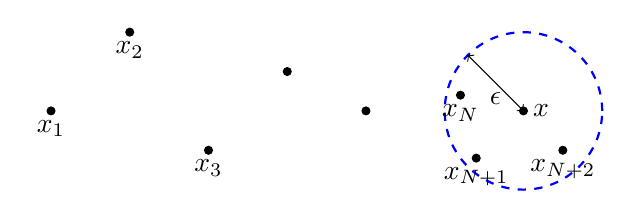
\begin{tikzpicture}
\draw[color=blue, dashed, thick](6,0) circle (1.0cm);
\draw[fill=black] (6,0) circle[radius=0.05cm] node [anchor=west] {$x$};
\draw[<->] (6,0) -- (5.29,0.71) node [midway, below] {$\epsilon$};

\draw[fill=black] (0,0) circle[radius=0.05cm] node [anchor=north] {$x_1$};
\draw[fill=black] (1,1) circle[radius=0.05cm] node [anchor=north] {$x_2$};
\draw[fill=black] (2,-0.5) circle[radius=0.05cm] node [anchor=north] {$x_3$};
\draw[fill=black] (3,0.5) circle[radius=0.05cm];
\draw[fill=black] (4,0) circle[radius=0.05cm];
\draw[fill=black] (5.2,0.2) circle[radius=0.05cm] node [anchor=north] {$x_N$};
\draw[fill=black] (5.4,-0.6) circle[radius=0.05cm] node [anchor=north] {$x_{N+1}$};
\draw[fill=black] (6.5,-0.5) circle[radius=0.05cm] node [anchor=north] {$x_{N+2}$};
\end{tikzpicture}
\caption{Convergence of sequence}
\end{figure}

\begin{remark}
This limit process conveys the intuitive idea that $x_n$ can be made arbitrarily close to $x$, provided that $n$ is sufficiently large. (Equivalently, if we remove more and more initial terms from the sequence, we see that the \emph{tail} of the sequence should be increasingly closer to $x$.)
\end{remark}

\begin{remark}
If $x_n\not\to x$, simply negate the definition for convergence:
\[\exists\epsilon>0,\quad\forall N\in\NN,\quad\exists n\ge N,\quad d(x_n,x)\ge\epsilon.\]
\end{remark}

\begin{remark}
From the definition, the convergence of a sequence depends not only on the sequence itself, but also on the metric space $X$. For instance, the sequence given by $a_n=\frac{1}{n}$ converges in $\RR$ (to $0$), but fails to converge in $\RR^+$. In cases of possible ambiguity, we shall specify ``convergent in $X$'' rather than ``convergent''. 
\end{remark}

\begin{example}
$\frac{1}{n}\to 0$.
\begin{proof}
Fix $\epsilon>0$. By the Archimedian property, there exists $N\in\NN$ such that $\frac{1}{N}<\epsilon$. Take $N=\floor{\frac{1}{\epsilon}}+1$. Then for all $n\ge N$,
\[\absolute{\frac{1}{n}-0}=\frac{1}{n}\le\frac{1}{N}=\frac{1}{\floor{\frac{1}{\epsilon}}+1}<\frac{1}{\frac{1}{\epsilon}}=\epsilon\]
as desired. Therefore $\frac{1}{n}\to0$.
\end{proof}
\end{example}

A useful tip for finding the required $N$ (in terms of $\epsilon$) is to work backwards from the result we wish to show, as illustrated in the following example.

\begin{example}
Let $a_n=1+(-1)^n\frac{1}{\sqrt{n}}$. Then $a_n\to 1$.

Before our proof, we aim to find some $N\in\NN$ such that if $n\ge N$ then
\begin{align*}
|a_n-1|&<\epsilon\\
\frac{1}{\sqrt{n}}=\absolute{(-1)^n\frac{1}{\sqrt{n}}}&<\epsilon\\
\frac{1}{n}&<\epsilon^2\\
n&>\frac{1}{\epsilon^2}
\end{align*}
Hence take $N=\floor{\frac{1}{\epsilon^2}}+1$.

\begin{proof}
Let $\epsilon>0$ be given. Take $N=\floor{\frac{1}{\epsilon^2}}+1$. If $n\ge N$, then
\begin{align*}
|a_n-1|&=\absolute{(-1)^n\frac{1}{\sqrt{n}}}=\frac{1}{\sqrt{n}}\\
&\le\frac{1}{\sqrt{N}}=\frac{1}{\sqrt{\floor{\frac{1}{\epsilon^2}}+1}}\\
&<\frac{1}{\sqrt{\frac{1}{\epsilon^2}}}=\epsilon
\end{align*}
as desired. Therefore $a_n\to1$.
\end{proof}
\end{example}

\begin{lemma}[Uniqueness of limit]
If a sequence converges, then its limit is unique.
\end{lemma}

\begin{proof}
Let $(x_n)$ be a sequence in $X$. Suppose that $x_n\to x$ and $x_n\to x^\prime$ for $x,x^\prime\in X$. We will show that $x^\prime=x$.

Let $\epsilon>0$ be given. Then there exists $N,N^\prime\in\NN$ such that
\begin{align*}
n\ge N&\implies d(x_n,x)<\frac{\epsilon}{2}\\
n\ge N^\prime&\implies d(x_n,x^\prime)<\frac{\epsilon}{2}
\end{align*}
Take $N_1\coloneqq\max\{N,N^\prime\}$. If $n\ge N_1$, then both hold. By the triangle inequality,
\[d(x,x^\prime)\le d(x,x_n)+d(x_n,x^\prime)<\frac{\epsilon}{2}+\frac{\epsilon}{2}=\epsilon.\]
Since this holds for all $\epsilon>0$, we must have $d(x,x^\prime)=0$. Hence $x=x^\prime$.
\end{proof}

Since the limit is unique, we can give it a notation.

\begin{notation}
If $(x_n)$ converges to $x$, we denote $\displaystyle\lim_{n\to\infty}x_n=x$.
\end{notation}

We now outline some important properties of convergent sequences in metric spaces.

\begin{proposition}
Let $(x_n)$ be a sequence in $X$.
\begin{enumerate}[label=(\roman*)]
\item $x_n\to x$ if and only if every open ball of $x$ contains $x_n$ for all but finitely many $n$.
\item If $(x_n)$ converges, then $(x_n)$ is bounded.
\item Suppose $E\subset X$. Then $x$ is a limit point of $E$ if and only if there exists a sequence $(x_n)$ in $E\setminus\{x\}$ such that $x_n\to x$.
\end{enumerate}
\end{proposition}

\begin{proof} \
\begin{enumerate}[label=(\roman*)]
\item \fbox{$\implies$} Suppose $x_n\to x$. Let $\epsilon>0$ be given, then there exists $N\in\NN$ such that
\[n\ge N\implies d(x_n,x)<\epsilon.\]
Corresponding to this $\epsilon$, consider the open ball $B_\epsilon(x)$. Then by definition, for $y\in X$, 
\[d(y,x)<\epsilon\implies y\in B_\epsilon(x).\]
Hence $n\ge N$ implies $x_n\in B_\epsilon(x)$.

\fbox{$\impliedby$} Suppose every open ball of $x$ contains all but finitely many of the $x_n$.

Let $\epsilon>0$ be given. Consider the open ball $B_\epsilon(x)$. Since $B_\epsilon(x)$ is a open ball of $x$, it will also eventually contain all $x_n$; that is, there exists $N\in\NN$ such that if $n\ge N$, then $x_n\in B_\epsilon(x)$, i.e. $d(x_n,x)<\epsilon$. Hence $x_n\to x$.

\item Suppose $x_n\to x$. Let $\epsilon>0$ be given. Then there exists $N\in\NN$ such that $n\ge N$ implies $d(x_n,x)<1$. Now let
\[r=\max\{1,d(x_1,x),\dots,d(x_N,x)\}.\]
Then $d(x_n,x)\le r$ for $n=1,2,\dots,N$, so the range of $x_n$ is bounded by $B_r(x)$. Hence $(x_n)$ is bounded.

\item \fbox{$\implies$} Suppose $x$ is a limit point of $E$. 

Consider a sequence of open balls $\brac{B_\frac{1}{n}(x)}$, for $n\in\NN$. Since $x$ is a limit point, each open ball intersects with $E$ at some point which is not $x$. We pick one such point $x_n$ from each $B_\frac{1}{n}(x)\cap E$. Then
\[d(x_n,x)<\frac{1}{n}.\]
Let $\epsilon>0$ be given. Then by the Archimedian property, there exists $N\in\NN$ such that $\frac{1}{N}<\epsilon$. If $n\ge N$,
\[d(x_n,x)\le\frac{1}{n}\le\frac{1}{N}<\epsilon,\]
which shows that $x_n\to x$.

\fbox{$\impliedby$} Suppose that there exists a sequence $(x_n)$ in $E\setminus\{x\}$ such that $x_n\to x$. Then for each open ball $B_\epsilon(x)$, we can find some $N\in\NN$ such that if $n\in\NN$ then
\[x_n\in B_\epsilon(x).\]
Since $x_n\in E\setminus\{x\}$, this shows that $x$ is a limit point of $E$.
\end{enumerate}
\end{proof}

\begin{proposition}[Ordering]
Suppose $(a_n)$ and $(b_n)$ are convergent sequences, and $a_n \le b_n$. Then
\[\lim_{n\to\infty}a_n\le\lim_{n\to\infty}b_n.\]
\end{proposition}

\begin{proof}
Let $\displaystyle a=\lim_{n\to\infty}a_n$, $\displaystyle b=\lim_{n\to\infty}b_n$. Suppose, for a contradiction, that $a>b$.

Let $\epsilon=a-b>0$ be given. There exists $N_1,N_2\in\NN$ such that
\begin{align*}
n\ge N_1&\implies|a_n-a|<\frac{\epsilon}{2},\\
n\ge N_2&\implies|b_n-b|<\frac{\epsilon}{2}.
\end{align*}
Let $N=\max\{N_1,N_2\}$, then $n\ge N$ implies
\[a_n>a-\frac{\epsilon}{2},\quad b_n<b+\frac{\epsilon}{2}\]
and thus
\[a_n-b_n>a-b-\epsilon=0\]
so $a_n>b_n$, which is a contradiction.
\end{proof}

\begin{remark}
If $a_n<b_n$, we may not necessarily have $\displaystyle\lim_{n\to\infty}a_n<\lim_{n\to\infty}b_n$. For instance, $-\frac{1}{n}<\frac{1}{n}$ but their limits are both $0$.
\end{remark}

\begin{proposition}[Arithmetic properties]
Suppose $(a_n)$ and $(b_n)$ are convergent seqeunces in $\CC$; let $\displaystyle a=\lim_{n\to\infty}a_n$, $\displaystyle b=\lim_{n\to\infty}b_n$. Then
\begin{enumerate}[label=(\roman*)]
\item $\displaystyle\lim_{n\to\infty}ca_n=ca$, where $c$ is a constant\hfill(scalar multiplication)
\item $\displaystyle\lim_{n\to\infty}(a_n+b_n)=a+b$\hfill(addition)
\item $\displaystyle\lim_{n\to\infty}(a_n b_n)=ab$\hfill(multiplication)
\item $\displaystyle\lim_{n\to\infty}\frac{a_n}{b_n}=\frac{a}{b}$ ($b_n\neq0$, $b\neq0$)\hfill(division)
\end{enumerate}
\end{proposition}

\begin{proof} \
\begin{enumerate}[label=(\roman*)]
\item The case where $c=0$ is trivial. Now suppose $c\neq0$. Let $\epsilon>0$ be given. Then there exists $N\in\NN$ such that
\[n\ge N\implies|a_n-a|<\frac{\epsilon}{|c|}.\]
Then if $n\ge N$,
\[|ca_n-ca|=|c|\:|a_n-a|<\epsilon.\]

\item Let $\epsilon>0$ be given. Since $a_n\to a$ and $b_n\to b$, there exists $N_1,N_2\in\NN$ such that
\begin{align*}
n\ge N_1&\implies|a_n-a|<\frac{\epsilon}{2},\\
n\ge N_2&\implies|b_n-b|<\frac{\epsilon}{2}.
\end{align*}
Let $N=\max\{N_1,N_2\}$, then $n\ge N$ implies
\begin{align*}
\absolute{(a_n+b_n)-(a+b)}
&\le|a_n-a|+|b_n-b|\\
&<\frac{\epsilon}{2}+\frac{\epsilon}{2}=\epsilon.
\end{align*}
Hence $\displaystyle\lim_{n\to\infty}(a_n+b_n)=a+b$, as desired.

\item Write
\[a_nb_n-ab=(a_n-a)(b_n-b)+a(b_n-b)+b(a_n-a).\]
Let $\epsilon>0$ be given. Since $a_n\to a$ and $b_n\to b$, there exist $N_1,N_2\in\NN$ such that
\begin{align*}
n\ge N_1&\implies|a_n-a|<\sqrt{\epsilon},\\
n\ge N_2&\implies|b_n-b|<\sqrt{\epsilon}.
\end{align*}
Let $N=\max\{N_1,N_2\}$. Then $n\ge N$ implies
\[|(a_n-a)(b_n-b)|<\epsilon,\]
and thus $\displaystyle\lim_{n\to\infty}(a_n-a)(b_n-b)=0$.

Note that $\displaystyle\lim_{n\to\infty}a(b_n-b)=\lim_{n\to\infty}b(a_n-a)=0$. Hence
\[\lim_{n\to\infty}(a_nb_n-ab)=0.\]

\item Since we have proven multiplication, it suffices to show that $\displaystyle\lim_{n\to\infty}\frac{1}{b_n}=\frac{1}{b}$.

Since $b_n\to b$, there exists $m\in\NN$ such that
\[n\ge m\implies|b_n-b|<\frac{1}{2}|b|.\]
Let $\epsilon>0$ be given. There exists $N\in\NN$, $N>m$ such that
\[n\ge N\implies|b_n-b|<\frac{1}{2}|b|^2\epsilon.\]
Hence for $n\ge N$,
\[\absolute{\frac{1}{b_n}-\frac{1}{b}}=\absolute{\frac{b-b_n}{b_nb}}<\frac{2}{|b|^2}|b_n-b|<\epsilon.\]
\end{enumerate}
\end{proof}

\begin{proposition}[Squeeze theorem]
Let $a_n\le c_n\le b_n$ where $(a_n)$ and $(b_n)$ are convergent sequences such that $\displaystyle\lim_{n\to\infty}a_n=\lim_{n\to\infty}b_n=L$. Then $(c_n)$ is also a convergent sequence, and
\[\lim_{n\to\infty}c_n=L.\]
\end{proposition}

\begin{proof}
Let $\epsilon>0$ be given. There exist $N_1,N_2\in\NN$ such that
\begin{align*}
n\ge N_1&\implies|a_n-L|<\epsilon,\\
n\ge N_2&\implies|b_n-L|<\epsilon.
\end{align*}
In particular, we have
\[a_n>L-\epsilon,\quad b_n<L+\epsilon.\]
Let $N=\max\{N_1,N_2\}$. Then $n\ge N$ implies
\[L-\epsilon<a_n\le c_n\le b_n<L+\epsilon\]
or
\[|c_n-L|<\epsilon.\]
Hence $(c_n)$ is convergent, and $c_n\to L$.
\end{proof}

Given a complex sequence $(z_n)$, there are two associated real sequences $\brac{\Re(z_n)}$ and $\brac{\Im(z_n)}$. The next result relates convergence of $(z_n)$ to convergence of $\brac{\Re(z_n)}$ and $\brac{\Im(z_n)}$.

\begin{proposition}[Complex sequences]
Let $(z_n)$ be a complex sequence. Write $z_n=x_n+iy_n$ with $x_n,y_n\in\RR$, so that $(x_n)$ and $(y_n)$ are real sequences. Then $(z_n)$ converges if and only if both $(x_n)$ and $(y_n)$ converge. Moreover, in the case where $(z_n)$ converges, we have
\[\lim_{n\to\infty}z_n=\lim_{x\to\infty}x_n+i\lim_{n\to\infty}y_n.\]
\end{proposition}
\pagebreak

\subsection{Subsequences}
\begin{definition}[Subsequence]
Given a sequence $(x_n)$, consider a sequence $(n_k)$ of positive integers such that $n_1<n_2<\cdots$. Then $(x_{n_k})$ is called a \vocab{subsequence}\index{subsequence} of $(x_n)$.

If $(x_{n_k})$ converges, its limit is called a \emph{subsequential limit} of $(x_n)$.
\end{definition}

\begin{proposition}
$(x_n)$ converges to $x$ if and only if every subsequence of $(x_n)$ converges to $x$.
\end{proposition}

\begin{proof} \

\fbox{$\implies$} Suppose $x_n\to x$. Let $\epsilon>0$ be give. Then there exists $N\in\NN$ such that
\[n\ge N\implies d(x_n,x)<\epsilon.\]
Every subsequence of $(x_n)$ can be written in the form $(x_{n_k})$ where $n_1<n_2<\cdots$ is a strictly increasing sequence of positive integers. Pick $M$ such that $n_M\ge N$. Then
\[k>M\implies n_k>n_M\ge N\implies d(x_{n_k},x)<\epsilon.\]
Hence every subsequence of $(x_n)$ converges to $x$.

\fbox{$\impliedby$} Suppose every subsequence of $(x_n)$ converges to $x$. Since $(x_n)$ is a subsequence of itself, we must have $x_n\to x$.
\end{proof}

\begin{proposition}
In a compact metric space, any sequence has a convergent subsequence.
\end{proposition}

\begin{proof}
Suppose $(x_n)$ is a sequence in a compact metric space $X$.

Let $E$ be the range of $(x_n)$. We have to consider two cases: (i) $E$ is finite, (ii) $E$ is infinite. For both cases, we will construct the desired convergent subsequence.
\begin{enumerate}[label=(\roman*)]
\item Notice that there are infinitely many terms in the sequence $(x_n)$, but only finitely many distinct terms in $E$. Hence by the pigeonhole principle, at least one term of $E$ appears infinitely many times in the sequence.

That is, there exists $x\in E$ and a sequence $(n_k)$ with $n_1<n_2<\cdots$ such that
\[x_{n_1}=x_{n_2}=\cdots=x.\]
This subsequence $(x_{n_k})$ that we have constructed evidently converges to $x$.

\item If $E$ is infinite, then $E$ is an infinite subset of a compact set. By \cref{prop:infinite-compact-lp}, $E$ has a limit point $x\in X$.

We now construct a subsequence $(x_{n_k})$ of $(x_n)$ such that $x_{n_k}\to x$. Choose $n_1$ so that $d(x,x_{n_1})<1$. Having chosen $n_1,\dots,n_{k-1}$, choose $n_k$ where $n_k>n_{k-1}$ such that $d(x,x_{n_k})<\frac{1}{k}$ (such $n_k$ exists due to \cref{prop:limit-point-inf-points}). Then $x_{n_k}\to x$.
\end{enumerate}
\end{proof}

\begin{corollary}[Bolzano--Weierstrass]
Every bounded sequence in $\RR^k$ has a convergent subsequence.
\end{corollary}

\begin{proof}
By \cref{prop:closed-bounded-compact-inf-lp}, every bounded sequence in $\RR^k$ lives in a compact subset of $\RR^k$, and therefore it lives in a compact metric space. Hence by the previous result, it contains a convergent subsequence converging to a point in $\RR^k$.
\end{proof}

\begin{lemma}
Suppose $(x_n)$ is a sequence in $X$. Then the subsequential limits of $(x_n)$ form a closed subset of $X$.
\end{lemma}

\begin{proof}
Let $E$ be the set of all subsequential limits of $(x_n)$, let $q$ be a limit point of $E$. We want to show that $q\in E$.

Choose $n_1$ so that $x_{n_1}\neq q$. (If no such $n_1$ exists, then $E$ has only one point, and there is nothing to prove.) Put $\delta=d(q,x_{n_1})$. Suppose $n_1,\dots,n_{i-1}$ are chosen. Since $q$ is a limit point of $E$, there is an $x\in E$ with $d(x,q)<2^{-1}\delta$. Since $x\in E$, there is an $n_i>n_{i-1}$ such that $d(x,x_{n_k})<2^{-i}\delta$. Thus
\[d(q,x_{n_k})<2^{1-i}\delta\]
for $i=1,2,3,\dots$. This says that $(x_{n_k})$ converges to $q$. Hence $q\in E$.
\end{proof}
\pagebreak

\subsection{Cauchy Sequences}
This is a very helpful way to determine whether a sequence is convergent or divergent, as it does not require the limit to be known. In the future you will see many instances where the convergence of all sorts of limits are compared with similar counterparts; generally we describe such properties as \emph{Cauchy criteria}.

\begin{definition}[Cauchy sequence]
A sequence $(x_n)$ in $X$ is a \vocab{Cauchy sequence}\index{Cauchy sequence} if 
\[\forall\epsilon>0,\quad\exists N\in\NN,\quad\forall n,m\ge N,\quad d(x_n,x_m)<\epsilon.\]
\end{definition}

\begin{remark}
Intuitively, we see that the distances between any two terms is sufficiently small after a certain point.
\end{remark}

A natural question is regarding the relationship between convergent sequences and Cauchy sequences. We now address this.

\begin{proposition} \
\begin{enumerate}[label=(\roman*)]
\item In any metric space, every convergent sequence is a Cauchy sequence.
\item If $X$ is a compact metric space and if $(x_n)$ is a Cauchy sequence in $X$, then $(x_n)$ converges to some point of $X$.
\item In $\RR^k$, every Cauchy sequence converges. 
\end{enumerate}
\end{proposition}

\begin{remark}
The converse of (i) is not true. For instance, the sequence $\{3,3.1,3.14,3.141,3.1415,\dots\}$ is a Cauchy sequence but does not converge in $\QQ$.
\end{remark}

\begin{proof} \
\begin{enumerate}[label=(\roman*)]
\item Suppose $x_n\to x$. Let $\epsilon>0$. There exists $N\in\NN$ such that for all $n\ge N$,
\[d(x_n,x)<\frac{\epsilon}{2}.\]
Then for all $n,m\ge N$,
\[d(x_n,x_m)\le d(x_n,x)+d(x_m,x)<\frac{\epsilon}{2}+\frac{\epsilon}{2}=\epsilon,\]
as desired. Hence $(x_n)$ is a Cauchy sequence.
\item Let $(x_n)$ be a Cauchy sequence in $X$. Since $X$ is compact, it is sequentially compact. Then there exists a subsequence $(x_{n_k})$ such that $x_{n_k}\to x$.
\begin{claim}
$x_n\to x$.
\end{claim}
Let $\epsilon>0$. Since $(x_n)$ is a Cauchy sequence, there exists $N_1\in\NN$ such that
\[n,m\ge N_1\implies d(x_n-x_m)<\frac{\epsilon}{2}.\]
$x_{n_k}\to x$ implies there exists $N_2\in\NN$ such that
\[n_k\ge N_2\implies d(x_{n_k},x)<\frac{\epsilon}{2}.\]
Let $N=\max\{N_1,N_2\}$, fix some $n_k\ge N$. Then $n\ge N$ implies
\[d(x_n,x)\le d(x_n,x_{n_k})+d(x_{n_k},x)<\frac{\epsilon}{2}+\frac{\epsilon}{2}=\epsilon.\]

\item Suppose $(x_n)$ is a Cauchy sequence.

We perform three steps:
\begin{itemize}
\item We first show that $(x_n)$ is bounded:

Pick $N\in\NN$ such that $|x_n-x_N|\le 1$ for all $n\ge N$. Then
\[|x_n|\le\max\{1+|x_N|,|x_1|,\dots,|x_{N-1}|\}.\]

\item Since $(x_n)$ is bounded, by Bolzano--Weierstrass, $(x_n)$ contains a subsequence $(x_{n_k})$ which converges to $x$.

\item We now show that $x_n\to x$.

Let $\epsilon>0$ be given. Since $(x_n)$ is a Cauchy sequence, there exists $N_1\in\NN$ such that
\[n,m\ge N_1\implies|x_n-x_m|<\frac{\epsilon}{2}.\]

Since $x_{n_k}\to x$, there exists $M\in\NN$ such that for all $k>M$,
\[n_k>n_M\implies |x_{n_k}-x|<\frac{\epsilon}{2}.\]
Now since $n_1<n_2<\cdots$ is a sequence of strictly increasing positive integers, we can pick $i>M$ such that $n_k>N_1$. Then for all $n\ge N_1$, by setting $m=n_k$ we obtain
\[ |x_n-x_{n_k}|<\frac{\epsilon}{2},\quad |x_{n_k}-x| < \frac{\epsilon}{2}.\]
Hence
\[|x_n-x|\le|x_n-x_{n_k}|+|x_{n_k}-x|<\epsilon.\]
Therefore $(x_n)$ is convergent, and $x_n\to x$.
\end{itemize}
\end{enumerate}
\end{proof}

\begin{definition}
A metric space $X$ is \vocab{complete} if every Cauchy sequence in $X$ converges.
\end{definition}

\begin{remark}
The above result shows that that all compact metric spaces and all Euclidean spaces are complete. It also implies that every closed subset $E$ of a complete metric space $X$ is complete. (Every Cauchy sequence in $E$ is a Cauchy sequence in $X$, hence it converges to some $x\in X$, and actually $x\in E$ since $E$ is closed.)
\end{remark}

\begin{example}
The sequence $(x_n)$ is defined as follows:
\[x_n=1+\frac{1}{2}+\cdots+\frac{1}{n}.\]
$(x_n)$ does not converge in $\RR$.
\begin{proof}
We claim that $(x_n)$ is not a Cauchy sequence. WLOG assume $n>m$. Consider
\[|x_n-x_m|=\frac{1}{m+1}+\frac{1}{m+2}+\cdots+\frac{1}{n}\ge\frac{n-m}{n}=1-\frac{m}{n}.\]
Let $n=2m$, then
\[|x_n-x_m|=|x_{2m}-x_m|>\frac{1}{2}.\]
Hence $(x_n)$ is not a Cauchy sequence, so it does not converge.
\end{proof}
\end{example}
\pagebreak

\subsection{Monotonic Sequences}
\begin{definition}[Monotonic sequence]
A sequence $(x_n)$ in $\RR$ is
\begin{enumerate}[label=(\roman*)]
\item \emph{monotonically increasing} if $x_n\le x_{n+1}$ for $n\in\NN$;
\item \emph{monotonically decreasing} if $x_n\ge x_{n+1}$ for $n\in\NN$;
\item \vocab{monotonic} if it is either monotonically increasing or monotonically decreasing.
\end{enumerate}
\end{definition}

\begin{lemma}[Monotone convergence theorem]
A monotonic sequence in $\RR$ converges if and only if it is bounded.
\end{lemma}

\begin{proof}
We show the case for monotically increasing sequences; the case for monotonically decreasing sequences is similar.

\fbox{$\implies$} We already proved that a convergent sequence is bounded.

\fbox{$\impliedby$} Suppose $(x_n)$ is a monotonically increasing sequence bounded above. Let $E$ be the range of $x_n$. Since $E$ is bounded above, let $x=\sup E$.
\begin{claim}
$x_n\to x$.
\end{claim}
By definition of supremum, $x_n\le x$ for all $n\in\NN$. For every $\epsilon>0$, there exists $N\in\NN$ such that
\[x-\epsilon<x_N\le x,\]
otherwise $x-\epsilon$ would be an upper bound of $E$. Since $(x_n)$ is monotically increasing, $n\ge N$ implies $x_N\le x_n\le x$, so 
\[x-\epsilon<x_n\le x,\]
which implies $|x_n-x|<\epsilon$. Hence $x_n\to x$.
\end{proof}
\pagebreak

\subsection{Limit Superior and Inferior}
For divergent sequences, we have the following definition.
\begin{definition}
Suppose $(x_n)$ is a sequence in $\RR$. We write $x_n\to\infty$ if
\[\forall M\in\RR,\quad\exists N\in\NN,\quad\forall n\ge N,\quad x_n\ge M.\]

Similarly, we write $x_n\to-\infty$ if 
\[\forall M\in\RR,\quad\exists N\in\NN,\quad\forall n\ge N,\quad x_n\le M.\]
\end{definition}

\begin{definition}
Suppose $(x_n)$ is a sequence in $\RR$. Let $E\subset\overline{\RR}$ be the set of all subsequential limits of $(x_n)$ (possibly including $+\infty$ and $-\infty$). Define 
\begin{align*}
\limsup_{n\to\infty}x_n&\coloneqq\sup E,\\
\liminf_{n\to\infty}x_n&\coloneqq\inf E,
\end{align*}
known as the \vocab{limit superior} and \vocab{limit infimum} of $(x_n)$ respectively.
\end{definition}

\begin{remark}
That is, limit superior is the ``largest'' subsequential limit; limit infimum is the ``smallest'' subsequential limit. 
\end{remark}

\begin{remark}
The limit superior and limit infimum exist due to the existence of supremum and infimum in $\overline{\RR}$.
\end{remark}

Equivalently, we can define limit superior (limit inferior) as the limit of supremum (infimum) of tails:
\begin{align*}
\limsup_{n\to\infty}x_n&=\lim_{n\to\infty}\brac{\sup_{k\ge n}x_k}\\
&=\lim_{n\to\infty}\brac{\sup\{a_n,a_{n+1},\dots\}}\\
\liminf_{n\to\infty}x_n&=\lim_{n\to\infty}\brac{\inf_{k\ge n}x_k}\\
&=\lim_{n\to\infty}\brac{\inf\{a_n,a_{n+1},\dots\}}\\
\end{align*}

\begin{proposition}
Suppose $(x_n)$ is a sequence in $\RR$. Then
\begin{enumerate}[label=(\roman*)]
\item $\displaystyle\limsup_{n\to\infty}x_n\in E$;
\item if $\displaystyle x>\limsup_{n\to\infty}x_n$, there exists $N\in\NN$ such that $x_n<x$ for all $n\ge N$.
\end{enumerate}
Moreover, $\displaystyle\limsup_{n\to\infty}x_n$ is the only number that satisfies (i) and (ii).
\end{proposition}

\begin{proof} \
\begin{enumerate}[label=(\roman*)]
\item We consider three cases for the value of $\displaystyle\limsup_{n\to\infty}x_n$:
\begin{itemize}
    \item If $\displaystyle\limsup_{n\to\infty}x_n=+\infty$, then $\sup E=+\infty$, so $E$ is not bounded above. Hence $(x_n)$ is not bounded above, so $(x_n)$ has a subsequence $(x_{n_k})$ such that $x_{n_k}\to\infty$
    \item If $\displaystyle\limsup_{n\to\infty}x_n\in\RR$, then $\sup E\in\RR$, so $E$ is bounded above. Hence at least one subsequential limit exists, so that (i) follows from Theorems 3.7 and 2.28.
    \item If $\displaystyle\limsup_{n\to\infty}x_n=-\infty$, then $\sup E=-\infty$, so $E$ contains only one element, namely $-\infty$. Hence $(x_n)$ has no subsequential limit. Thus for any $M\in\RR$, $x_n>M$ for at most a finite number of values of $n$, so that $x_n\to-\infty$.
\end{itemize}
\item We prove by contradiction.

Suppose there is a number $\displaystyle x>\limsup_{n\to\infty}x_n$ such that $x_n\ge x$ for infinitely many values of $n$. In that case, there is a number $y\in E$ such that $\displaystyle y\ge x>\limsup_{n\to\infty}x_n$, contradicting the definition of $\displaystyle\limsup_{n\to\infty}x_n$.
\end{enumerate}

We now show uniqueness. Suppose, for a contradiction, that two numbers $p$ and $q$ satisfy (i) and (ii). WLOG assume $p<q$. Then choose $x$ such that $p<x<q$. Since $p$ satisfies (i), we have $x_n<x$ for all $n\ge N$. But then $q$ cannot satisfy (i).
\end{proof}

Of course, an analogous result is true for $\displaystyle\liminf_{n\to\infty}x_n$. 

\begin{example}
\begin{itemize}
\item Let $(x_n)$ be a sequence containing all rationals. Then every real number is a subsequential limit, and 
\[\limsup_{n\to\infty}x_n=+\infty,\quad\liminf_{n\to\infty}=-\infty.\]

\item Let $x_n=\dfrac{(-1)^n}{1+\frac{1}{n}}$. Then
\[\limsup_{n\to\infty}x_n=1,\quad\liminf_{n\to\infty}x_n=-1.\]

\item For a seqeunce $(x_n)$ in $\RR$, $x_n\to x$ if and only if
\[\limsup_{n\to\infty}x_n=\liminf_{n\to\infty}x_n=x.\]
\end{itemize}
\end{example}

\begin{proposition}\label{prop:limsup-liminf-comp}
If $a_n\le b_n$ for $n\ge N$ where $N$ is fixed, then
\begin{align*}
\liminf_{n\to\infty}a_n&\le\liminf_{n\to\infty}b_n,\\
\limsup_{n\to\infty}a_n&\le\limsup_{n\to\infty}b_n.
\end{align*}
\end{proposition}

\begin{proposition}[Arithmetic properties] \
\begin{enumerate}[label=(\roman*)]
\item If $k>0$, $\displaystyle\limsup_{n\to\infty}ka_n=k\limsup_{n\to\infty}a_n$.

If $k<0$, $\displaystyle\limsup_{n\to\infty}ka_n=k\liminf_{n\to\infty}a_n$.

\item $\displaystyle\limsup(a_n+b_n)\le\limsup a_n+\limsup b_n$

Moreover, $\displaystyle\limsup_{n\to\infty}(a_n+b_n)$ may be bounded from below as follows:
\[ \limsup_{n\to\infty}(a_n+b_n)\ge\limsup_{n\to\infty}a_n+\liminf_{n\to\infty}b_n.\]

write down the analogous properties for liminf, and to prove (i) and (ii)
\end{enumerate}
\end{proposition}

Now you should try to prove (i) for liminf as well; as for (ii), try to explain why properties (i),(ii) for limsup and property (i) for liminf would imply property (ii) for liminf
\pagebreak

\section{Series}
\begin{definition}[Series]
Given a sequence $(a_n)$, we associate a sequence $(s_n)$, where
\[s_n=\sum_{k=1}^n a_k=a_1+a_2+\cdots+a_n,\]
where the term $s_n$ is called the \emph{$n$-th partial sum}. The sequence $(s_n)$ is often written as
\[\sum_{n=1}^{\infty}a_n,\]
which we call a \vocab{series}.
\end{definition}

\begin{definition}[Convergence of series]
We say that the series \emph{converges} if $s_n\to s$ (the sequence of partial sums converges), and write $\displaystyle\sum_{n=1}^\infty a_n=s$; that is,
\[\forall\epsilon>0,\quad\exists N\in\NN,\quad\forall n\ge N,\quad\absolute{\sum_{k=1}^n a_k-s}<\epsilon.\]
The number $s$ is called the \emph{sum} of the series. If $(s_n)$ diverges, the series is said to \emph{diverge}.
\end{definition}

\begin{notation}
When there is no possible ambiguity, we write $\displaystyle\sum_{n=1}^{\infty}a_n$ simply as $\sum a_n$.
\end{notation}

The Cauchy criterion can be restated in the following form:

\begin{proposition}[Cauchy criterion]
$\sum a_n$ converges if and only if
\[\forall\epsilon>0,\quad\exists N\in\NN,\quad\forall n\ge m\ge N,\quad\absolute{\sum_{k=m}^n a_k}\le\epsilon.\]
\end{proposition}
\pagebreak

\subsection{Convergence Tests}
To determine the convergence of a series, apart from using the definition and the Cauchy criterion, we also have the following methods:
\begin{itemize}
\item Divergence test (\cref{lemma:divergence-test})
\item Boundedness of partial sums (\cref{lemma:bounded-partial-sums}, for series of non-negative terms)
\item Comparison test (\cref{lemma:comparison-test})
\item Root test (\cref{lemma:root-test})
\item Ratio test (\cref{lemma:ratio-test})
\item Absolute convergence (\cref{lemma:absolute-convergence})
\end{itemize}

\begin{lemma}[Divergence test]\label{lemma:divergence-test}
If $a_n\not\to0$, then $\sum a_n$ diverges.
\end{lemma}

\begin{proof}
We prove the contrapositive: if $\sum a_n$ converges, then $a_n\to0$.

In the Cauchy criterion, take $m=n$, then $|a_n|\le\epsilon$ for all $n\ge N$.
\end{proof}

\begin{remark}
The converse is not true; a counterexample of the harmonic series.
\end{remark}

\begin{lemma}\label{lemma:bounded-partial-sums}
A series of non-negative terms converges if and only if its partial sums form a bounded sequence.
\end{lemma}

\begin{proof}
Partial sums are monotonically increasing. But bounded monotonic sequences converge.
\end{proof}

\begin{lemma}[Comparison test]\label{lemma:comparison-test}
Consider two sequences $(a_n)$ and $(b_n)$.
\begin{enumerate}[label=(\roman*)]
\item Suppose $|a_n|\le b_n$ for all $n\ge N_0$ (where $N_0$ is some fixed integer). If $\sum b_n$ converges, then $\sum a_n$ converges.
\item Suppose $a_n\ge b_n\ge0$ for all $n\ge N_0$. If $\sum b_n$ diverges, then $\sum a_n$ diverges.
\end{enumerate}
\end{lemma}

\begin{proof} \
\begin{enumerate}[label=(\roman*)]
\item Since $\sum b_n$ converges, by the Cauchy criterion, fix $\epsilon>0$, there exists $N\in\NN$, $N\ge N_0$ such that for $n\ge m\ge N$,
\[\sum_{k=m}^{n}b_k\le\epsilon.\]
By the triangle inequality,
\[\absolute{\sum_{k=m}^{n}a_k}\le\sum_{k=m}^{n}|a_k|\le\sum_{k=m}^{n}b_k\le\epsilon,\]
so $\sum a_n$ converges, by the Cauchy criterion.

\item We prove the contrapositive. If $\sum a_n$ converges, and since $|b_n|\le a_n$ for all $n\ge N_0$, then by (i), $\sum b_n$ converges.
\end{enumerate}
\end{proof}

To employ the comparison test, we need to be familiar with several series whose convergence or divergence is known.

\begin{example}[Geometric series]
A geometric series takes the form
\[\sum_{n=0}^{\infty}x^n.\]

\begin{proposition*} \
\begin{enumerate}[label=(\roman*)]
\item If $|x|<1$, then $\sum x^n$ converges;
\[\sum_{n=0}^{\infty}x^n=\frac{1}{1-x}.\]
\item If $|x|\ge1$, then $\sum x^n$ diverges.
\end{enumerate}
\end{proposition*}

\begin{proof} \
\begin{enumerate}[label=(\roman*)]
\item For $|x|<1$, the $n$-th partial sum is given by
\begin{equation*}\tag{1}
\sum_{k=0}^{n}x^k=1+x+x^2+\cdots+x^n.
\end{equation*}
Multiplying both sides of (1) by $x$ gives
\begin{equation*}\tag{2}
x\sum_{k=0}^{n}x^k=x+x^2+x^3\cdots+x^{n+1}.
\end{equation*}
Taking the difference of (1) and (2),
\[(1-x)\sum_{k=0}^{n}x^k=1-x^{n+1}\]a
nd so
\[\sum_{k=0}^{n}x^k=\frac{1-x^{n+1}}{1-x}.\]
Taking limits $n\to\infty$, the result follows.

\item For $|x|\ge 1$, $x^n\not\to 0$. By the divergence test, $\sum x^n$ diverges.
\end{enumerate}
\end{proof}
\end{example}

\begin{example}[$p$-series]
A $p$-series takes the form
\[\sum_{n=1}^{\infty}\frac{1}{n^p}.\]
To determine the convergence of $p$-series, we first prove the following lemma, which states that a rather ``thin'' subsequence of $(a_n)$ determines the convergence of $\sum a_n$.

\begin{lemma*}[Cauchy condensation test]
Suppose $a_1\ge a_2\ge\cdots\ge0$. Then $\sum a_n$ converges if and only if the series
\[\sum_{k=0}^{\infty}2^ka_{2^k}=a_1+2a_2+4a_4+\cdots\]
converges.
\end{lemma*}

\begin{proof}
Let $s_n$ and $t_k$ denote the $n$-th partial sum of $(a_n)$ and the $k$-th partial sum of $(2^ka_{2^k})$ respectively; that is,
\begin{align*}
s_n&=a_1+a_2+\cdots+a_n,\\
t_k&=a_1+2a_2+\cdots+2^ka_{2^k}.
\end{align*}
We consider two cases:
\begin{itemize}
\item For $n<2^k$, group terms to give
\begin{align*}
s_n&=a_1+a_2+\cdots+a_n\\
&\le a_1+(a_2+a_3)+\cdots+(a_{2^k}+\cdots+a_{2^{k+1}-1})\\
&\le a_1+2a_2+\cdots+2^ka_{2^k}\\
&=t_k.
\end{align*}
By comparison test, if $(t_k)$ converges, then $(s_n)$ converges.
%Thus if $(s_n)$ is unbounded, then $(t_k)$ is unbounded.

\item For $n>2^k$,
\begin{align*}
s_n&\ge a_1+a_2+(a_3+a_4)+\cdots+(a_{2^{k-1}+1}+\cdots+a_{2^k})\\
&\ge\frac{1}{2}a_1+a_2+2a_4+\cdots+2^{k-1}a_{2^k}\\
&=\frac{1}{2}t_k.
\end{align*}
By comparison test, if $(s_n)$ converges, then $(t_k)$ converges.
%Thus if $(t_k)$ is unbounded, then $(s_n)$ is unbounded.
\end{itemize}
\end{proof}

\begin{proposition*}[$p$-test] \
\begin{enumerate}[label=(\roman*)]
\item If $p>1$, $\sum\frac{1}{n^p}$ converges.
\item If $p\le1$, $\sum\frac{1}{n^p}$ diverges.
\end{enumerate}
\end{proposition*}

\begin{proof}
Note that if $p\le0$, then $\frac{1}{n^p}\not\to0$. By the divergence test, $\sum\frac{1}{n^p}$ diverges.

If $p>0$, we want to apply the above lemma. Consider the series
\[\sum_{k=0}^{\infty}2^k\cdot\frac{1}{(2^k)^p}=\sum_{k=0}^{\infty}2^{(1-p)k}=\sum_{k=0}^{\infty}\brac{2^{1-p}}^k,\]
which is a geometric series. Hence the above series converges if and only if $|2^{1-p}|<1$, which holds if and only if $1-p<0$. Then apply the above lemma to conclude the convergence of $\frac{1}{n^p}$.
\end{proof}

\begin{remark}
If $p=1$, the resulting series is known as the \emph{harmonic series} (which diverges). If $p=2$, the resulting series converges, and the sum of this series is $\frac{\pi^2}{6}$ (Basel problem).
\end{remark}
\end{example}

\begin{example}[The number $e$]
Consider the series
\[\sum_{n=0}^{\infty}\frac{1}{n!}.\]
\begin{claim}
The above series converges.
\end{claim}
Consider the $n$-th partial sum:
\begin{align*}
\sum_{k=0}^{n}\frac{1}{k!}
&=\frac{1}{0!}+\frac{1}{1!}+\frac{1}{2!}+\frac{1}{3!}+\cdots+\frac{1}{n!}\\
&\le1+1+\frac{1}{2}+\frac{1}{2^2}+\cdots+\frac{1}{2^{n-1}}\\
&<1+1+\frac{1}{2}+\frac{1}{2^2}+\cdots=3.
\end{align*}
Since the partial sums are bounded (by $3$), and the terms are non-negative, the series converges. Then we can make the following definition for the sum of the series:
\[e\coloneqq\sum_{n=0}^\infty\frac{1}{n!}\]

\begin{proposition*}
$e$ is irrational.
\end{proposition*}

\begin{proof}
Suppose, for a contradiction, that $e$ is rational. Then $e=\frac{p}{q}$, where $p$ and $q$ are positive integers. Let $s_n$ denote the $n$-th partial sum:
\[s_n=\sum_{k=0}^{n}\frac{1}{k!}.\]
Then
\begin{align*}
e-s_n
&=\frac{1}{(n+1)!}+\frac{1}{(n+2)!}+\frac{1}{(n+3)!}+\cdots\\
&<\frac{1}{(n+1)!}\brac{1+\frac{1}{n+1}+\frac{1}{(n+1)^2}+\cdots}\\
&=\frac{1}{(n+1)!}\cdot\frac{n+1}{n}=\frac{1}{n!n}
\end{align*}
and thus
\[0<e-s_n<\frac{1}{n!n}.\]
Taking $n=q$ and multiplying both sides by $q!$ gives
\[0<q!(e-s_q)<\frac{1}{q}.\]
Note that $q!e$ is an integer (by assumption), and
\[q!s_q=q!\brac{1+1+\frac{1}{2!}+\cdots+\frac{1}{q!}}\]
is an integer, so $q!(e-s_n)$ is an integer. Since $q\ge1$, this implies the existence of an integer between $0$ and $1$, which is absurd. Hence we have reached a contradiction.
\end{proof}

\begin{lemma*}
$e$ is equivalent to the following:
\[\lim_{n\to\infty}\brac{1+\frac{1}{n}}^n=e.\]
\end{lemma*}

\begin{proof}
Let
\[s_n=\sum_{k=0}^n\frac{1}{k!},\quad t_n=\brac{1+\frac{1}{n}}^n.\]
By the binomial theorem,
\[t_n=1+1+\frac{1}{2!}\brac{1-\frac{1}{n}}+\frac{1}{3!}\brac{1-\frac{1}{n}}\brac{1-\frac{2}{n}}+\cdots+\frac{1}{n!}\brac{1-\frac{1}{n}}\brac{1-\frac{2}{n}}\cdots\brac{1-\frac{n-1}{n}}.\]
Comparing term by term, we see that $t_n\le s_n$. By \cref{prop:limsup-liminf-comp}, we have that
\[\limsup_{n\to\infty}t_n\le\limsup_{n\to\infty}s_n=e.\]

Next, if $n\ge m$,
\[t_n\ge1+1+\frac{1}{2!}\brac{1-\frac{1}{n}}+\cdots+\frac{1}{m!}\brac{1-\frac{1}{n}}\cdots\brac{1-\frac{m-1}{n}}.\]
Let $n\to\infty$, keeping $m$ fixed. We get
\[\liminf_{n\to\infty}t_n\ge1+1+\frac{1}{2!}+\cdots+\frac{1}{m!},\]
so that
\[s_m\le\liminf_{n\to\infty}t_n.\]
Letting $m\to\infty$, we finally get
\[e\le\liminf_{n\to\infty}t_n.\]

\end{proof}
\end{example}

\begin{lemma}[Root test]\label{lemma:root-test}
Given $\sum a_n$, let $\displaystyle\alpha=\limsup_{n\to\infty}\sqrt[n]{|a_n|}$.
\begin{enumerate}[label=(\roman*)]
\item If $\alpha<1$, $\sum a_n$ converges.
\item If $\alpha>1$, $\sum a_n$ diverges.
\item If $\alpha=1$, the test gives no information.
\end{enumerate}
\end{lemma}

\begin{remark}
We use limsup since the limsup of a sequence always exists (in $\overline{\RR}$), while the limit may not necessarily exist.
\end{remark}

\begin{proof} \
\begin{enumerate}[label=(\roman*)]
\item If $\alpha<1$, choose $\beta$ such that $\alpha<\beta<1$. Since $\displaystyle\beta>\limsup_{n\to\infty}\sqrt[n]{|a_n|}$, there exists $n\in\NN$ such that for all $n\ge N$,
\[\sqrt[n]{|a_n|}<\beta,\]
or
\[|a_n|<\beta^n.\]
Note that $\sum\beta^n$ converges since $0<\beta<1$. By the comparison test, $\sum a_n$ converges.

\item If $\alpha>1$, $\displaystyle\limsup_{n\to\infty}\sqrt[n]{|a_n|}>1$, so there exists a subsequence $(a_{n_k})$ such that
\[\sqrt[n_k]{|a_{n_k}|}\to\alpha.\]
Thus $|a_n|>1$ for infinitely many values of $n$. Hence $a_n\not\to0$, so by the divergence test, $\sum a_n$ diverges.

\item Consider the series $\sum\frac{1}{n}$ and $\sum\frac{1}{n^2}$. For each of these series $\alpha=1$, but the first diverges, the second converges. Hence the condition that $\alpha=1$ does not give us information on the convergence of a series.
\end{enumerate}
\end{proof}

\begin{lemma}[Ratio test]\label{lemma:ratio-test}
The series $\sum a_n$
\begin{enumerate}[label=(\roman*)]
\item converges if $\displaystyle\limsup_{n\to\infty}\absolute{\frac{a_{n+1}}{a_n}}<1$;
\item diverges if $\displaystyle\absolute{\frac{a_{n+1}}{a_n}}\ge1$ for all $n\ge N_0$ (where $N_0$ is some fixed integer).
\end{enumerate}
\end{lemma}

\begin{proof} \
\begin{enumerate}[label=(\roman*)]
\item If $\displaystyle\limsup_{n\to\infty}\absolute{\frac{a_{n+1}}{a_n}}<1$, there exists $\beta<1$ and $N\in\NN$ such tht for all $n\ge N$,
\[\absolute{\frac{a_{n+1}}{a_n}}<\beta.\]
In particular, from $n=N$ to $n=N+k$,
\begin{align*}
|a_{N+1}|&<\beta|a_N|\\
|a_{N+2}|&<\beta|a_{N+1}|<\beta^2|a_N|\\
&\vdots\\
|a_{N+k}|&<\beta^k|a_N|
\end{align*}
Hence for all $n\ge N$,
\begin{align*}
|a_n|&<|a_N|\beta^{n-N}\\
&=\brac{|a_N|\beta^{-N}}\beta^n
\end{align*}
and taking the sum gives
\[\sum|a_n|<|a_N|\beta^{-N}\sum\beta^n.\]
Since $\beta<1$, $\sum\beta^n$ converges. By the comparison test, $\sum a_n$ converges.

\item Suppose $\displaystyle\absolute{\frac{a_{n+1}}{a_n}}\ge1$ for all $n\ge N_0$. Then $|a_{n+1}|\ge|a_n|$ for $n\ge N_0$, so $a_n\not\to0$. By the divergence test, $\sum a_n$ diverges.
\end{enumerate}
\end{proof}

\begin{remark}
The ratio test is easier to apply than the root test (since it is usually easier to compute ratios than $n$-th roots), but the root test is more powerful, as shown by Theorem 3.37 of \cite{rudin}.
\end{remark}

The series $\sum a_n$ is said to \emph{converge absolutely} if the series $\sum|a_n|$ converges.

\begin{lemma}[Absolute convergence]\label{lemma:absolute-convergence}
If $\sum a_n$ converges absolutely, then $\sum a_n$ converges.
\end{lemma}

\begin{proof}
Suppose $\sum a_n$ converges absolutely; that is, $\sum|a_n|$ converges. Using the Cauchy criterion, fix $\epsilon>0$, there exists $N\in\NN$ such that for all $n\ge m\ge N$,
\[\absolute{\sum_{k=m}^{n}|a_k|}<\epsilon.\]
Since all the terms are non-negative, we can simply write
\[\sum_{k=m}^{n}|a_k|<\epsilon.\]
By the triangle inequality,
\[\absolute{\sum_{k=m}^{n}a_k}\le\sum_{k=m}^{n}|a_k|<\epsilon.\]
Hence by the Cauchy criterion, $\sum a_n$ converges.
\end{proof}

Note that the converse may not necessarily be true. We say that $\sum a_n$ is \emph{conditionally convergent} if it converges, but does not converge absolutely.

\begin{example}
The alternating harmonic series given by
\[\sum_{n=1}^{\infty}\frac{(-1)^{n+1}}{n}\]
converges to $\ln 2$, but it is not absolutely convergent (since the harmonic series diverges).
\end{example}
\pagebreak

\subsection{Summation by Parts}
\begin{proposition}[Partial summation formula]\label{prop:part-sum-formula}
Given two sequences $(a_n)$ and $(b_n)$, let the $n$-partial sum of $(a_n)$ be denoted by
\[A_n=\sum_{k=0}^{n}a_k\]
for $n\ge0$; let $A_{-1}=0$. Then, if $0\le p\le q$, we have
\[\sum_{n=p}^{q}a_nb_n=\sum_{n=p}^{q-1}A_n(b_n-b_{n+1})+A_qb_q-A_{p-1}b_p.\]
\end{proposition}

\begin{proof}
The RHS can be written as
\begin{align*}
&\sum_{n=p}^{q-1}A_nb_n+A_qb_q-\sum_{n=p}^{q-1}A_nb_{n+1}-A_{p-1}b_p\\
&=\sum_{n=p}^{q}A_nb_n-\sum_{n=p-1}^{q-1}A_nb_{n+1}\\
&=\sum_{n=p}^{q}A_nb_n-\sum_{n=p}^{q}A_{n-1}b_n\\
&=\sum_{n=p}^{q}\brac{A_n-A_{n-1}}b_n\\
&=\sum_{n=p}^{q}a_nb_n
\end{align*}
which is equal to the LHS.
\end{proof}

\begin{proposition}\label{prop:part-sum-limit}
Suppose $(a_n)$ and $(b_n)$ are sequences such that
\begin{itemize}
\item the partial sums $A_n$ of $\sum a_n$ form a bounded sequence,
\item $b_0\ge b_1\ge b_2\ge\cdots$,
\item $b_n\to0$.
\end{itemize}
Then $\sum a_nb_n=0$.
\end{proposition}

\begin{proof}
Since the partial sums $A_n$ form a bounded sequence, there exists $M$ such that
\[|A_n|\le M\quad(\forall n\in\NN)\]
Since $b_n\to0$, fix $\epsilon>0$, there exists $N\in\NN$ such that
\[b_N\le\frac{\epsilon}{2M}.\]
For $q\ge p\ge N$, by the partial summation formula, we have
\begin{align*}
\absolute{\sum_{n=p}^{q}a_nb_n}
&=\absolute{\sum_{n=p}^{q-1}A_n(b_n-b_{n+1})+A_qb_q-A_{p-1}b_p}\\
&\le M\absolute{\sum_{n=p}^{q-1}(b_n-b_{n+1})+b_q+b_p}\quad[\because |A_n|\le M]\\
&=M\absolute{(b_p-b_q)+b_q+b_p}=2Mb_p\le 2Mb_n\le\epsilon.
\end{align*}
By the Cauchy criterion, $\sum a_nb_n$ converges to $0$.
\end{proof}

\begin{corollary}[Alternating series test]
Suppose $(c_n)$ is a sequence such that
\begin{itemize}
\item $|c_1|\ge|c_2|\ge|c_3|\ge\cdots$,
\item $c_{2m-1}\ge0,c_{2m}\le0$ for $m=1,2,3,\dots$,
\item $c_n\to0$.
\end{itemize}
Then $\sum c_n=0$.
\end{corollary}

\begin{proof}
Let
\[a_n=(-1)^{n+1},\quad b_n=|c_n|.\]
Note that
\begin{itemize}
\item the partial sums of $(a_n)$ are 0s and 1s, so they are bounded;
\item $b_0\ge b_1\ge b_2\ge\cdots$ holds by assumption;
\item $c_n\to0$ implies $|c_n|\to0$, so $b_n\to0$.
\end{itemize}
Then by \cref{prop:part-sum-limit}, we have that $\sum a_nb_n=0$, so $\sum c_n=0$.
\end{proof}
\pagebreak

\subsection{Addition and Multiplication of Series}
\begin{proposition}
If $\sum a_n=A$ and $\sum b_n=B$, then
\begin{enumerate}[label=(\roman*)]
\item $\sum(a_n+b_n)=A+B$,\hfill(addition)
\item $\sum ca_n=cA$ for some constant $c$.\hfill(scalar multiplication)
\end{enumerate}
\end{proposition}

\begin{proof} \
\begin{enumerate}[label=(\roman*)]
\item Let the $n$-th partial sums be denoted by
\[A_n=\sum_{k=0}^{n}a_k,\quad B_n=\sum_{k=0}^{n}b_k.\]
Then
\[\lim_{n\to\infty}\sum_{k=0}^{n}(a_k+b_k)=\lim_{n\to\infty}(A_n+B_n)=\lim_{n\to\infty}A_n+\lim_{n\to\infty}B_n=A+B.\]
\item Simply factor out the constant $c$:
\[\lim_{n\to\infty}\sum_{k=0}^{n}ca_k=c\lim_{n\to\infty}\sum_{k=0}^{n}a_k=cA.\]
\end{enumerate}
\end{proof}

The situation becomes more complicated when we consider multiplication of two series. To begin with, we have to define the product. This can be done in several ways; we shall consider the so-called ``Cauchy product''. 

\begin{definition}[Cauchy product]
Given $\sum a_n$ and $\sum b_n$, let
\[c_n=\sum_{k=0}^{n}a_k b_{n-k}\quad(n=0,1,2,\dots)\]
We call $\sum c_n$ the \emph{product} of the two given series.
\end{definition}

This definition may be motivated as follows. If we take two power series $\sum a_nz^n$ and $\sum b_nz^n$, multiply them term by term, and collect terms containing the same power of $z$, we get
\begin{align*}
\brac{\sum_{n=0}^{\infty}a_nz^n}\brac{\sum_{n=0}^{\infty}b_nz^n}
&=\brac{a_0+a_1z+a_2z^2+\cdots}\brac{b_0+b_1z+b_2z^2+\cdots}\\
&=a_0b_0+(a_0b_1+a_1b_0)z+(a_0b_2+a_1b_1+a_2b_0)z^2+\cdots\\
&=c_0+c_1z+c_2z^2+\cdots
\end{align*}
Setting $z=1$, we arrive at the above definition.

Note that $\sum c_n$ may not converge, even if $\sum a_n$ and $\sum b_n$ do. However $\sum c_n$ converges if an additional condition is imposed: at least one of the two series converges absolutely.

\begin{proposition}[Mertens' theorem]
Suppose $\sum a_n=A$, $\sum b_n=B$, and $\sum a_n$ converges absolutely. Then their Cauchy product converges to $AB$.
\end{proposition}

\begin{proof}
Let $\sum c_n$ be the Cauchy product of $\sum a_n$ and $\sum b_n$. Let the $n$-th partial sums be denoted by
\[A_n=\sum_{k=0}^{n}a_k,\quad B_n=\sum_{k=0}^{n}b_k,\quad C_n=\sum_{k=0}^{n}c_k.\]
Also let $\beta_n=B_n-B$. Then 
\begin{align*}
C_n&=a_0b_0+(a_0b_1+a_1b_0)+\cdots+(a_0b_n+a_1b_{n-1}+\cdots+a_nb_0)\\
&=a_0B_n+a_1B_{n-1}+\cdots+a_nB_0\\
&=a_0(B+\beta_n)+a_1(B+\beta_{n-1})+\cdots+a_n(B+\beta_0)\\
&=A_nB+(a_0\beta_n+a_1\beta_{n-1}+\cdots+a_n\beta_0)
\end{align*}
Our goal is to show that $C_n\to AB$. Since $A_nB\to AB$, it suffices to show that
\[\gamma_n=a_0\beta_n+a_1\beta_{n-1}+\cdots+a_n\beta_0\to0.\]

We now use the absolute convergence of $(a_n)$; let $\alpha=\sum|a_n|$. Fix $\epsilon>0$, there exists $N_1\in\NN$ such that
\[n\ge N_1\implies \sum_{k=0}^{n}|a_k|-\alpha<\epsilon\]
since the terms are non-negative. Since $B_n\to B$, $\beta_n\to0$. Then there exists $N_2\in\NN$ such that
\[n\ge N_2\implies|\beta_n|\le\epsilon.\]
Let $N=\max\{N_1,N_2\}$. Then for $n\ge N$, by triangle inequality,
\begin{align*}
|\gamma_n|&=|\beta_0 a_n+\cdots+\beta_n a_0|\\
&\le|\beta_0a_n+\cdots+\beta_Na_{n-N}|+|\beta_{N+1}a_{n-N-1}+\cdots+\beta_na_0|\\
&\le|\beta_0a_n+\cdots+\beta_Na_{n-N}|+\epsilon(|a_{n-N-1}|+\cdots+|a_0|)\\
&\le|\beta_0a_n+\cdots+\beta_Na_{n-N}|+\epsilon\alpha.
\end{align*}
Keeping $N$ fixed, and letting $n\to\infty$, we get
\[\limsup_{n\to\infty}|\gamma_n|\le\epsilon\alpha,\]
sine $a_n\to0$. Since $\epsilon$ is arbitrary, we have $\gamma_n\to0$, as desired.
\end{proof}

\begin{proposition}[Abel's theorem]
Let $\sum a_n=A$, $\sum b_n=B$, $\sum c_n=C$, where $\sum c_n$ is the Cauchy product of $\sum a_n$ and $\sum b_n$. Then $C=AB$.
\end{proposition}
\pagebreak

\subsection{Rearrangements}
\begin{definition}[Rearrangement]
Let $(k_n)$ be a sequence in which every positive integer appears once and only once. Let
\[a_n^\prime=a_{k_n}\quad(\forall n\in\NN)\]
We say that $\sum a_n^\prime$ is a \emph{rearrangement} of $\sum a_n$.
\end{definition}

If $(s_n)$ and $(s_n^\prime)$ are the sequences of partial sums of $(a_n)$ and $(a_n^\prime)$ respectively, it is easily seen that, in general, these two sequences consist of entirely different numbers. We are thus led to the problem of determining under what conditions all rearrangements of a convergent series will converge and whether the sums are necessarily the same.

\begin{proposition}[Riemann]
Let $\sum a_n$ be a series of real numbers which converges, but not absolutely. Suppose $-\infty\le\alpha\le\beta\le\infty$. Then there exists a rearrangement $\sum a_n^\prime$ with partial sums $s_n^\prime$ such that
\[\liminf_{n\to\infty}s_n^\prime=\alpha,\quad\limsup_{n\to\infty}s_n^\prime=\beta.\]
\end{proposition}

\begin{proof}
\todo{to do}
\end{proof}

\begin{proposition}
If $\sum a_n$ is a series of complex numbers which converges absolutely, then every rearrangement of $\sum a_n$ converges, and they all converge to the same sum.
\end{proposition}
\pagebreak

\section*{Exercises}
\addcontentsline{toc}{section}{Exercises}
\begin{exercise}
Show the following:
\begin{enumerate}[label=(\roman*)]
\item $\displaystyle\lim_{n\to\infty}\frac{1}{n^p}=0$ ($p>0$)
\item $\displaystyle\lim_{n\to\infty}\sqrt[n]{p}=1$ ($p>0$)
\item $\displaystyle\lim_{n\to\infty}\sqrt[n]{n}=1$
\item $\displaystyle\lim_{n\to\infty}\frac{n^\alpha}{(1+p)^n}=0$ ($p>0$, $\alpha\in\RR$)
\item $\displaystyle\lim_{n\to\infty}x^n=0$ ($|x|<1$)
\end{enumerate}
\end{exercise}

\begin{solution} \
\begin{enumerate}[label=(\roman*)]
\item Let $\epsilon>0$ be given. Take $N=\floor{\brac{\frac{1}{\epsilon}}^\frac{1}{p}}+1$. Then $n\ge N$ implies
\[\absolute{\frac{1}{n^p}-0}=\frac{1}{n^p}\le\frac{1}{N^p}<\frac{1}{\brac{\brac{\frac{1}{\epsilon}}^\frac{1}{p}}^p}=\epsilon.\]
\item We need to consider the cases when $p>1$, $p=1$, and $0<p<1$.

If $p>1$, 

\item 
\item 
\item 
\end{enumerate}
\end{solution}

\begin{exercise}
Let $(x_n)$ be a sequence in $\RR$, let $\alpha\ge2$ be a constant. Define the sequence $(y_n)$ as follows:
\[y_n=x_n+\alpha x_{n+1}\quad(n=1,2,\dots)\]
Show that if $(y_n)$ is convergent, then $(x_n)$ is also convergent.
\end{exercise}

\begin{exercise}[\cite{rudin} 3.1]
Prove that the convergence of $(x_n)$ implies the convergence of $(|x_n|)$. Is the converse true?
\end{exercise}

\begin{solution}
Let $\epsilon>0$ be given. Since $(x_n)$ is a Cauchy sequence, there exists $N\in\NN$ such that for all $n,m\ge N$,
\[|x_n-x_m|<\epsilon.\]
See that
\[\absolute{|x_n|-|x_m|}\le|x_n-x_m|<\epsilon,\]
so $(|x_n|)$ is a Cauchy sequence, and therefore must converge.

The converse is not true, as shown by the sequence $(x_n)$ with $x_n=(-1)^n$.
\end{solution}

\begin{exercise}[\cite{rudin} 3.3]
The sequence $(x_n)$ is recursively defined by
\[\begin{cases}
x_0=\sqrt{2},\\
x_{n+1}=\sqrt{2+x_n}\quad n\ge0.
\end{cases}\]
Show that $(x_n)$ converges.
\end{exercise}

\begin{solution}
We first prove by induction that $x_n\le x_{n+1}\le 2$ for all $n\in\NN$. For $n=0$,
\[x_0=\sqrt{2}\le\sqrt{2+\sqrt{2}}=x_1\le\sqrt{2+\sqrt{4}}=2.\]
If $x_{n-1}\le x_n\le 2$, then
\[x_n=\sqrt{2+x_{n-1}}\le\sqrt{2+x_n}=x_{n+1}\le\sqrt{2+2}=2.\]
Hence $(x_n)$ is monotonically increasing and bounded above by $2$. By the monotone convergence theorem, $(x_n)$ converges; let $x_n\to x$. Applying the limit on both sides of $x_{n+1}=\sqrt{2+x_n}$,
\begin{align*}
\lim_{n\to\infty}x_{n+1}&=\lim_{n\to\infty}\sqrt{2+x_n}\\
x&=\sqrt{2+x}\\
x&=2\text{ or }1
\end{align*}
Since all $x_n\ge0$, we must have $x=2$.
\end{solution}

\begin{exercise}[Contractive sequence]
A sequence $(x_n)$ in $\RR$ is \emph{contractive} if there exists $k\in[0,1)$ such that
\[|x_{n+2}-x_{n+1}|\le k|x_{n+1}-x_n|\quad(\forall n\in\NN)\]
Show that every contractive sequence is convergent.
\end{exercise}

\begin{solution}
By induction on $n$, we have
\[|a_{n+1}-a_n|\le k^{n-1}|a_2-a_1|\quad(\forall n\in\NN)\]
Thus
\begin{align*}
|a_{n+p}-a_{n}|&\le|a_{n+1}-a_{n}|+|a_{n+2}-a_{n+1}|+\cdots+|a_{n+p}-a_{n+p-1}|\\ 
&\le\brac{k^{n-1}+k^{n}+\cdots+k^{n+p-2}}|a_{2}-a_{1}|\\ 
&\le k^{n-1}\brac{1+k+k^{2}+\cdots+k^{p-1}}|a_{2}-a_{1}|\\ 
&\le\frac{k^{n-1}}{1-k}|a_{2}-a_{1}|
\end{align*}
for all $n,p\in\NN$. Since $k^{n-1}\to0$ as $n\to\infty$ (independently of $p$), this implies $(a_n)$ is a Cauchy sequence (in $\RR$) and, hence, it is convergent.
\end{solution}

\begin{exercise}[\cite{rudin} 3.4]
Find the limit superior and limit inferior of the sequence $(x_n)$ defined by
\[x_1=0,\quad x_{2m}=\frac{x_{2m-1}}{2},\quad x_{2m+1}=x_{2m}+\frac{1}{2}.\]
\end{exercise}

\begin{solution}
We shall prove by induction that
\[x_{2m}=\frac{1}{2}-\frac{1}{2^m},\quad x_{2m+1}=1-\frac{1}{2^m}\]
for $m=1,2,\dots$. The second of these equalities is a direct consequence of the first, and so we need only prove the first. Immediate computation shows that $x_2=0$ and $x_3=\frac{1}{2}$. Hence assume that both formulae holds for $m\le r$. Then
\[x_{2r+2}=\frac{1}{2}x_{2r+1}=\frac{1}{2}\brac{1-\frac{1}{2^r}}=\frac{1}{2}-\frac{1}{2^{r+1}}.\]
This completes the induction. We thus have $\displaystyle\limsup_{n\to\infty}x_n=1$ and $\displaystyle\liminf_{n\to\infty}x_n=\frac{1}{2}$.
\end{solution}

\begin{exercise}[\cite{rudin} 3.7]
Prove that the convergence of $\sum a_n$ implies the convergence of
\[\sum\frac{\sqrt{a_n}}{n}\]
if $a_n\ge0$.
\end{exercise}

\begin{exercise}[\cite{rudin} 3.8]
If $\sum a_n$ converges, and if $(b_n)$ is monotonic and bounded, prove that $\sum a_nb_n$ converges.
\end{exercise}

\begin{exercise}[\cite{rudin} 3.13]
Prove that the Cauchy product of two absolutely convergent series converges absolutely.
\end{exercise}

\begin{exercise}[\cite{rudin} 3.23]
Suppose $(p_n)$ and $(q_n)$ are Cauchy sequences in a metric space $X$. Show that the sequence $\brac{d(p_n,q_n)}$ converges.
\end{exercise}